Statistics is the science of planning studies and experiments, obtaining data, organizing, summarizing, presenting, analyzing, and interpreting those data and then drawing conclusions based on them; particularly among its main applications, the \emph{descriptive statistics} is a branch that comprises a set of methods which aim to describe relevant characteristics in data \cite{triola2017elementary}. The descriptive statistics methods either employ graphical elements such as boxplots, histograms, bar graphs and scatter plots to analyze data or yield numerical summary measures such as means, standard deviations, correlation coefficients and other related indices \cite{devore2011probability}. The methods that compose a descriptive statistical approach for data analysis are simple yet powerful tools that play a very important role within the scope of this project. The \emph{kurtosis} and the \emph{z-score} are the most prominent measurements for the application and will be clearly explained after some basic concepts. The graphical methods are irrelevant for this work.

Chapter~\ref{chapter:materials_and_methods} will provide information about the nature of data to be analysed in this work. The concepts of \emph{population}, \emph{sample} and \emph{variable} are elementary: a population is a well-defined collection of objects that might be included in the analysis, a sample is a subset of a population and a variable is a feature of the objects which may change from one object to another \cite{devore2011probability}. Moreover, a \emph{frequency distribution} is a tool that presents how the data is partitioned among several categories by listing each category and its frequency of data values in each of them; a \emph{relative frequency distribution} is a frequency distribution where each frequency is represented by a proportion, usually as percentage \cite{triola2017elementary}.

\subsection{Measures of Central Tendency}

According to \citeonline{mendenhall2016statistics}, the measures of central tendency provides several ways to locate the center of the relative frequency distribution, and the three most common are the \emph{arithmetic mean}, i.e. the average of the measurements, the \emph{median}, i.e. the middle number when the measurements are ordered in ascending or descending order and the \emph{mode}, i.e. the value that occurs with the greatest frequency. Figure \ref{fig:central_tendency} presents the interpretations of these three metrics for a relative frequency distribution:

\begin{figure}[H]
	\centering
	\caption{\label{fig:central_tendency} Examples of the mean (a), median (b) and mode (c) for a relative frequency distribution.}
	\begin{center}
    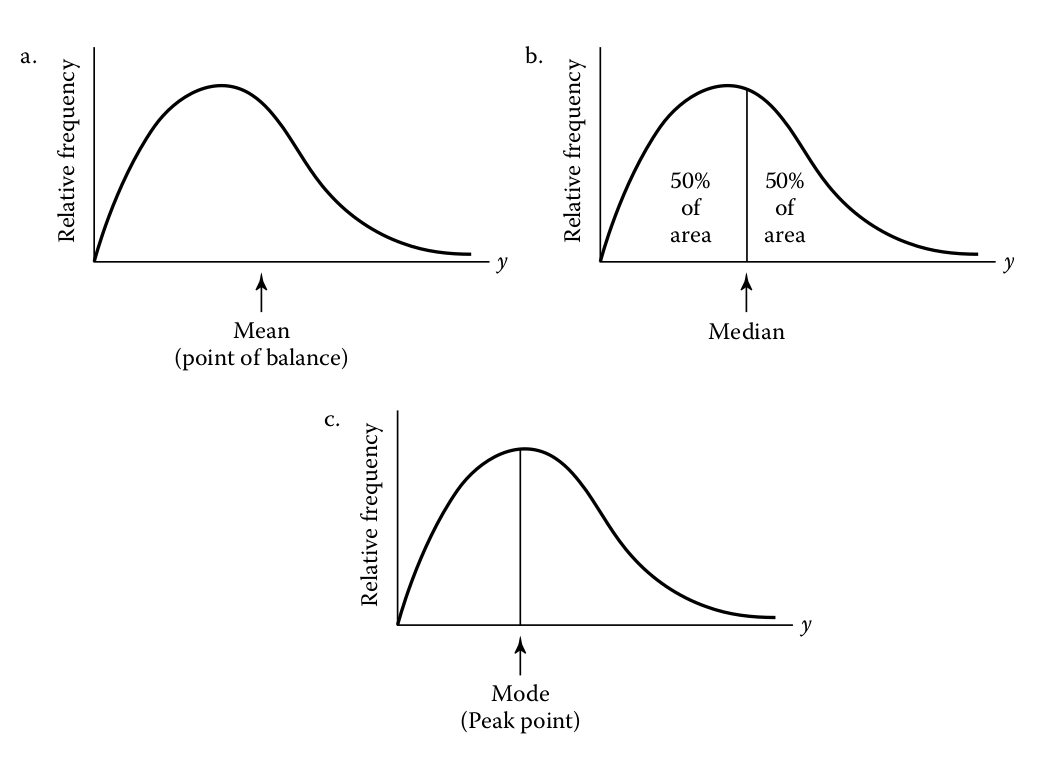
\includegraphics[scale=0.4]{images/central_tendency.png}
	\end{center}
	\centering
    \fadaptada{mendenhall2016statistics}
\end{figure}

Mathematically, the arithmetic mean is given by

\begin{equation}
\label{eqn:arithmetic_mean}
\bar{x} = \frac{1}{n} \sum_{i=1}^{n} x_{i} = \frac{x_{1} + x_{2} + \dots + x_{n}}{n},
\end{equation}

\noindent where $n$ is the sample size and $x_{i}$ represents the $i$-th observation of the variable $x$ \cite{zwillinger1999crc}.

\subsection{Measures of Variation}

The measures of variation provide a description of how the values spread along the distribution, and commonly used measures are the range, the variance, and the standard deviation \cite{mendenhall2016statistics}. The range is simply the difference between the largest and the smallest value within the data, which may precisely point out its variability, since it does not comprise the middle values among the distribution \cite{devore2011probability}. The variance and the standard deviation are closely related, as the former measures variability based on the squared deviations about
the mean and the latter is the positive square root of the variance, as

\begin{align}
\label{eqn:variance_std}
\sigma^{2} = \frac{1}{n - 1} \sum_{i = 1}^{n} \left(x_{i} - \bar{x}\right)^{2}
&&
\sigma = \sqrt{\sigma^{2}},
\end{align}

\noindent where $\sigma^{2}$ and $\sigma$ are respectively the variance and the standard deviation, $x_{i}$ is the $i$-th observation of the variable $x$, $\bar{x}$ is the mean, all concerning a sample or the population \cite{zwillinger1999crc}.

\subsection{Measures of Relative Standing}

The measures of the relative standing of an observation describe its location among other values in the distribution, and two examples of these measures are \emph{percentiles} and \emph{z-scores} \cite{mendenhall2016statistics}. Percentiles are values that split the data into 100 parts in a sorted dataset, so that the $i$-th percentile stands for the $i(n + 1) / 100$ observation, e.g. the $25$-th percentile comprises $25\%$ of the data; the $z$-score, or standard score, is given by

\begin{equation}
\label{eqn:z_score}
z = \frac{x_{i} - \bar{x}}{\sigma},
\end{equation}

\noindent where $x_{i}$ is the $i$-th observation of the variable $x$, $\bar{x}$ is the mean and $\sigma$ is the standard deviation of the population or the sample \cite{zwillinger1999crc}.

\subsection{Probability Distributions}

Probability is a common and natural concept among human life, used in expressions such as ``It probably will be cold tonight''; however, there is no common formal definition accepted among statisticians and related researchers \cite{degroot2012probability}. The study of randomness, variability and uncertainty in populations is done by analyzing probabilities, i.e. numerical descriptions of how likely an event is to occur \cite{devore2011probability}. Some basic concepts that support the probability theory are described also to the light of \citeonline{devore2011probability}, as follows:

\begin{itemize}
    \item \emph{Experiment}: Any activity or process whose outcome is subject to uncertainty;
    
    \item \emph{Sample Space}: The sample space of an experiment is the set of all possible outcomes for it;
    
    \item \emph{Event}: Any collection or subset of outcomes of a sample space;
    
    \item \emph{Random Variable}: Any rule that associates a number with each outcome in a sample space of some experiment; mathematically, it is a function with the sample space as its domain and the real numbers as its range;
    
    \item \emph{Discrete Random Variable}: A random variable with a finite set or a countable infinite sequence of possible values;
    
    \item \emph{Continuous Random Variable}: A random variable that yields zero as the probability for every possible outcome or its set of possible values are in a single interval of the real line or all numbers in a disjoint union of intervals.
    
\end{itemize}

From these concepts, it is possible to define a distribution in the scope of the probability theory. The \emph{probability distribution} is a collection of all probabilities computed from a  discrete or continuous random variable with the set of real numbers; a \emph{discrete} probability distribution is represented by the probability function itself, while a \emph{continuous} probability distribution is represented by a \sigla{p.d.f}{probability density function} \cite{mendenhall2016statistics}.

\subsection{Kurtosis}

The \emph{kurtosis} is one of the probability distribution shape statistics, which measures the extent of the peak in a distribution, i.e. its ``peakedness''; smaller absolute values indicate that the distribution tends to be uniform \cite{zwillinger1999crc}. First of all, the concepts of \emph{expectation} and \emph{moments} should be described. The expectation of a random variable (and consequently, of a distribution) is a value that summarizes its nature and is given by

\begin{align}
\label{eqn:expectation}
E(X) = \int_{-\infty}^{\infty} x p(x)dx
&&
E(X) = \sum_{x} x p(x),
\end{align}

\noindent where $x$ is each possible outcome of the random variable $X$, $p(x)$ is the probability density function for a continuous random variable (left) and the probability function for a discrete random variable (right) \cite{degroot2012probability}. Still according to \citeonline{degroot2012probability}, for a random variable $X$ and every positive $k \in \mathbb{R}$, the expectation $E(X^{k})$ is
called the $k$-th moment of $X$. The $r$-th moment may be described, according to \citeonline{zwillinger1999crc}, as

\begin{equation}
\label{eqn:rth_moment}
m_{r} = \frac{1}{n}
        \sum_{i=1}^{k}p_{i}(x_{i} - \bar{x})^{r}
\end{equation}

\noindent for every $x_{i}$ in the possible outcomes of $X$. Thus, kurtosis may be defined as the ratio of the fourth moment (equation \ref{eqn:rth_moment} with $r = 4$) by the square of the variance (also equation \ref{eqn:rth_moment} with $r = 2$), denoted by

\begin{equation}
\label{eqn:kurtosis}
g_{2} = \frac{m_{4}}{(m_{2})^{2}} - 3
\end{equation}

The $-3$ constant is due to Fischer's approach, where the kurtosis of a normal distribution is zero.